\documentclass[../MasterThesis.tex]{subfiles}
\graphicspath{ {./assets/images/} }


%----------------------------------------------------------------------------
%----------------------------------------------------------------------------

\begin{document}
	
	

%---------------------------------------------------------------------------
\newpage
%---------------------------------------------------------------------------

\section{Technical Background} \label{subsection:technicalbackground}




%---------------------------------
\subsection{Melt}

The Melt framework (MLT/Melt) is a multimedia framework as a command-line (CLI) tool that can be used for video editing and playback. It is written in C and provides a set of tools, libraries, and services for handling multimedia content, including video and audio.~\cite{melt} 


A variety of tasks can be performed with Melt, including the application of filters on audio or video files, and converting data between different formats. 

In the following, the structure of the Melt framework will be briefly explained. For this, the documentation~\cite{melt}  as well as the actual code of the framework\myfootcite{melt_code} are taken into consideration.

\textit{Producer}, \textit{Consumer} and \textit{MLT frame objects} are fundamental components in the Melt framework.

A \textit{MLT frame object} is a data structure that is used for representing multimedia content. 
It is a container that holds multimedia data. Each \textit{MLT frame object} contains a single uncompressed frame image and its associated audio samples. These frame objects can be processed individually, which allows the user to manipulate and transform multimedia content efficiently.
\textit{MLT frame objects} can store the multimedia data in various formats and they support metadata annotations, which allows to attach additional information or properties to the multimedia content. This includes filters, which are discussed in Section \ref{subsection:meltfilter}.


A \textit{Producer} generates or provides data -- it produces the \textit{MLT Frame objects}. 
It reads data from files or other data sources. The \textit{Producer} serves as the starting point of the data processing pipeline in Melt. It retrieves the raw data and passes it on to other components, for example the \textit{Consumer}. This can be seen in Figure \ref{fig:producer_consumer}.

A \textit{Consumer} requests \textit{MLT Frame objects} from the producer.
It is responsible for consuming or processing the data that was produced by the \textit{Producer} or other components that are between the \textit{Producer} and \textit{Consumer}. 
The \textit{Consumer} represents the endpoint of the data processing pipeline and produces the final output or results.



\begin{figure}[H]
	\centering
	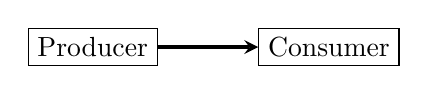
\begin{tikzpicture}
		% Nodes
		\node[draw, rectangle] (producer) at (0,0) {Producer};
		\node[draw, rectangle] (consumer) at (3,0) {Consumer};
		% Arrows
		\draw[->,>=stealth, line width=1.2pt] (producer) -- (consumer);
	\end{tikzpicture}
	\caption{Producer-Consumer Relationship}
	\label{fig:producer_consumer}
\end{figure}

Applying filters in the Melt framework is a technique for manipulating multimedia content, including videos. 
Melt filters can perform a wide range of operations, including colour correction, blurring, sharpening, cropping, resizing, and many others. A list of the filters can be found on the Melt website.\myfootcite{melt_filters}

To apply a filter in Melt, a filter instance has to be created and its parameters have to contain the name of the filter and, if needed, the filter parameters and values for those.

Filters are processing units that manipulate the multimedia data as it flows through the pipeline. They are placed between the producer and consumer, allowing them to modify the data before it reaches the consumer. This can be seen in Figure \ref{fig:producer_filter_consumer}.



\begin{figure}[H]
	\centering
	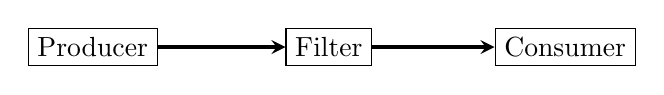
\begin{tikzpicture}
		% Nodes
		\node[draw, rectangle] (producer) at (0,0) {Producer};
		\node[draw, rectangle] (filter) at (3,0) {Filter};
		\node[draw, rectangle] (consumer) at (6,0) {Consumer};
		% Arrows
		\draw[->,>=stealth, line width=1.2pt] (producer) -- (filter);
		\draw[->,>=stealth, line width=1.2pt] (filter) -- (consumer);
	\end{tikzpicture}
	\caption{Producer-Filter-Consumer Relationship}
	\label{fig:producer_filter_consumer}
\end{figure}












\newpage
%-------------------------------------------------------------------------------------------------------
\subsection{Melt Filter Comparison} \label{subsection:meltfilter}

The goal for this thesis project is to adjust the RGB values of a video with sliders. For this purpose, various Melt filters that seemed suitable were examined and compared to identify the most suitable ones for implementing this functionality. RGB colour representation was described in Section~\ref{subsection:RGB}.

In the following, a selection of filters, that influence the RGB representation of the video are listed. This includes the filter name, description and possible parameters from the Melt website.\myfootcite{melt_filters}
Those filters were then executed locally, to compare the visual results of applying them.


\begin{table}[H]
	\footnotesize
	\begin{tabular}{lp{4.1cm}p{4.1cm}}
		\toprule
		Name & Description & Parameters \\
		\midrule
		\texttt{avfilter.colorbalance} & Adjust the colour balance & \texttt{av.rs}: set red shadows \newline \texttt{av.gs}: set green shadows \\
		\texttt{avfilter.colorchannelmixer} & Adjust colours by mixing color channels & \\
		\texttt{avfilter.colorcontrast} & Adjust colour contrast between RGB components & \\
		\texttt{frei0r.coloradj\_RGB} & Simple colour adjustment & \\
		\bottomrule
	\end{tabular}
\end{table}




% TODO: List and compare different filters and their results

Use of \texttt{avfilter.colorchannelmixer}:

\url{https://www.mltframework.org/plugins/FilterAvfilter-colorchannelmixer/}

\texttt{title: colorchannelmixer \newline
	media types: Video \newline
	description: Adjust colors by mixing color channels.}

Execution of \texttt{melt https://s3.eu-central-1.amazonaws.com/accurate-player\--demo-assets/timecode/sintel-2048-timecode-stereo.mp4 \\ -filter avfilter.colorbalance av.rs=1 av.gm=1 av.bh=1}:


\begin{minipage}{0.5\textwidth}
	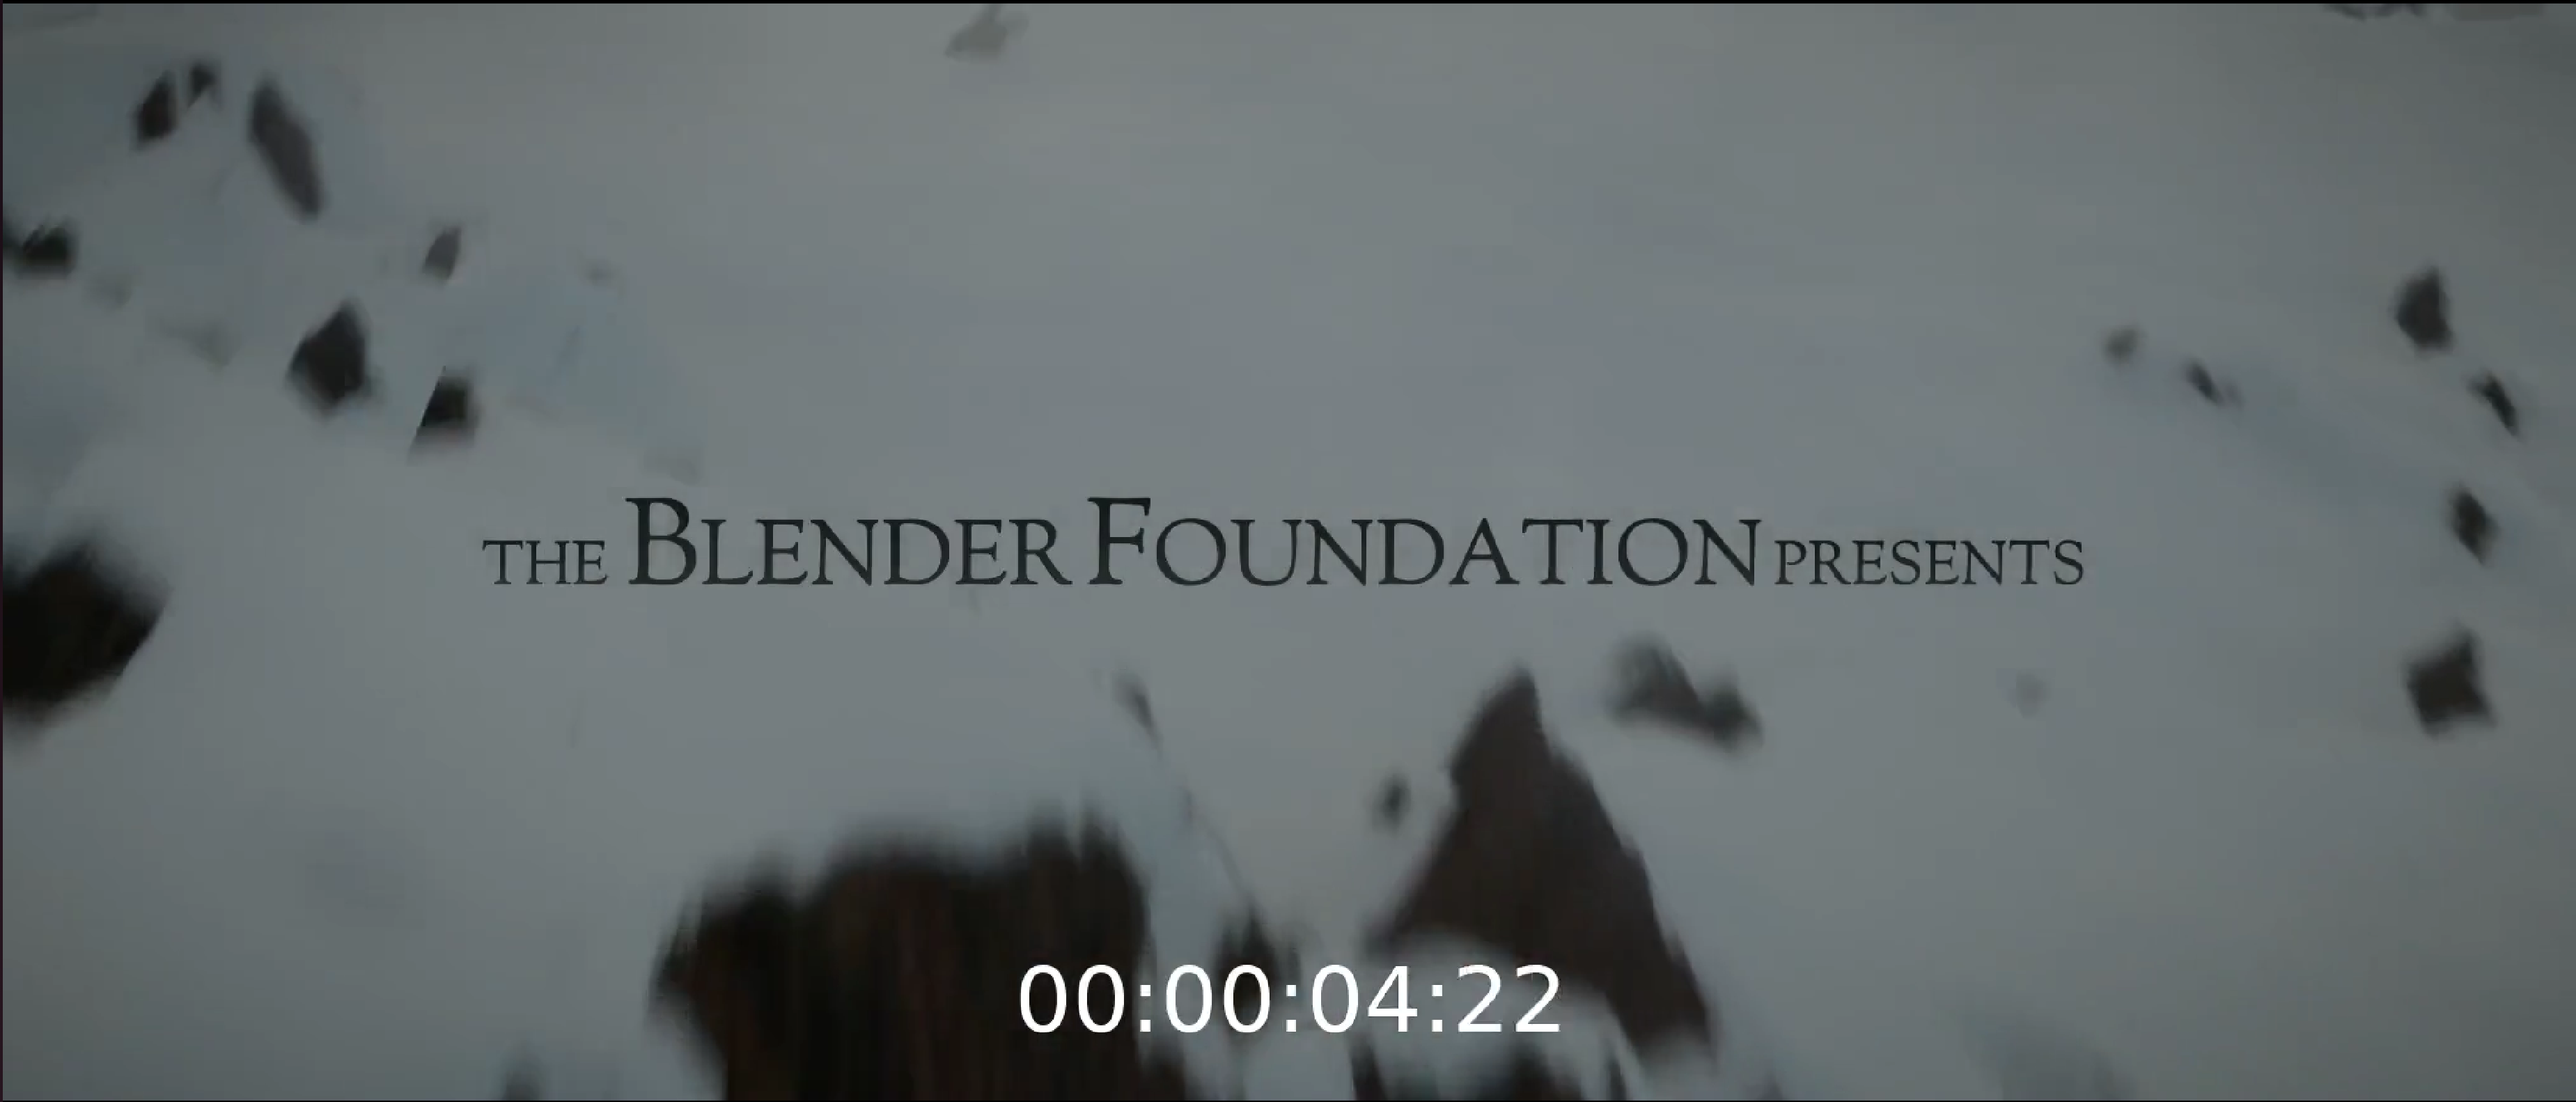
\includegraphics[width=0.9\textwidth]{colourdefault.png}
	Original colours
\end{minipage}\begin{minipage}{0.5\textwidth}
	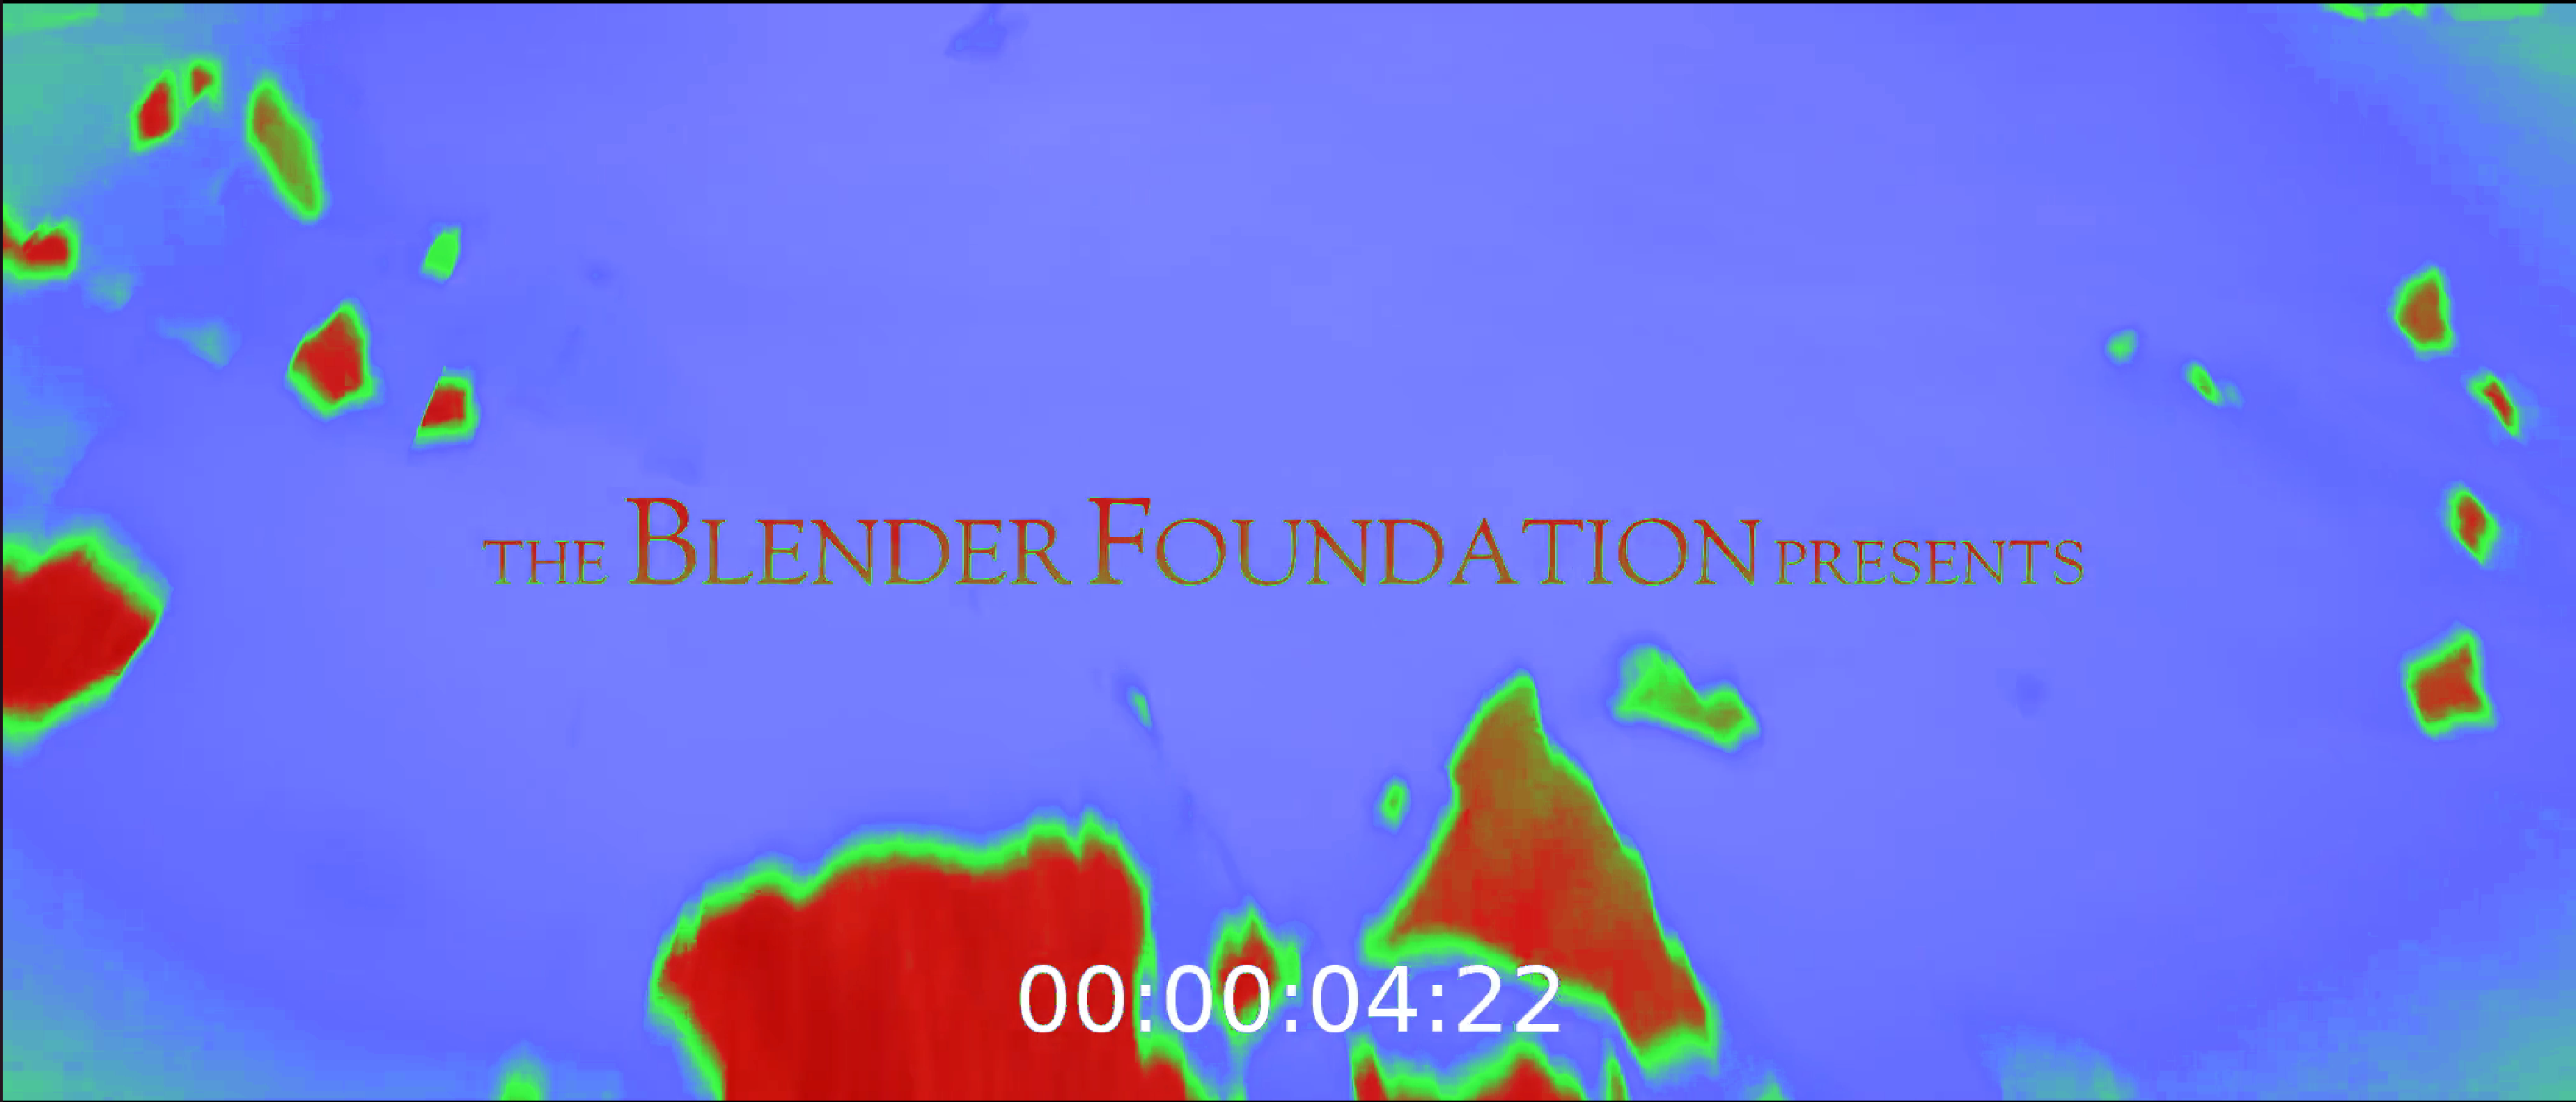
\includegraphics[width=0.9\textwidth]{colourhigh.png}
	Colours with \texttt{av.rs=1} \texttt{av.gm=1} \texttt{av.bh=1}
\end{minipage}

Adding filter to \texttt{local\_melt.py} to execute it in the Accurate Player using JIT:
`
\begin{center}
	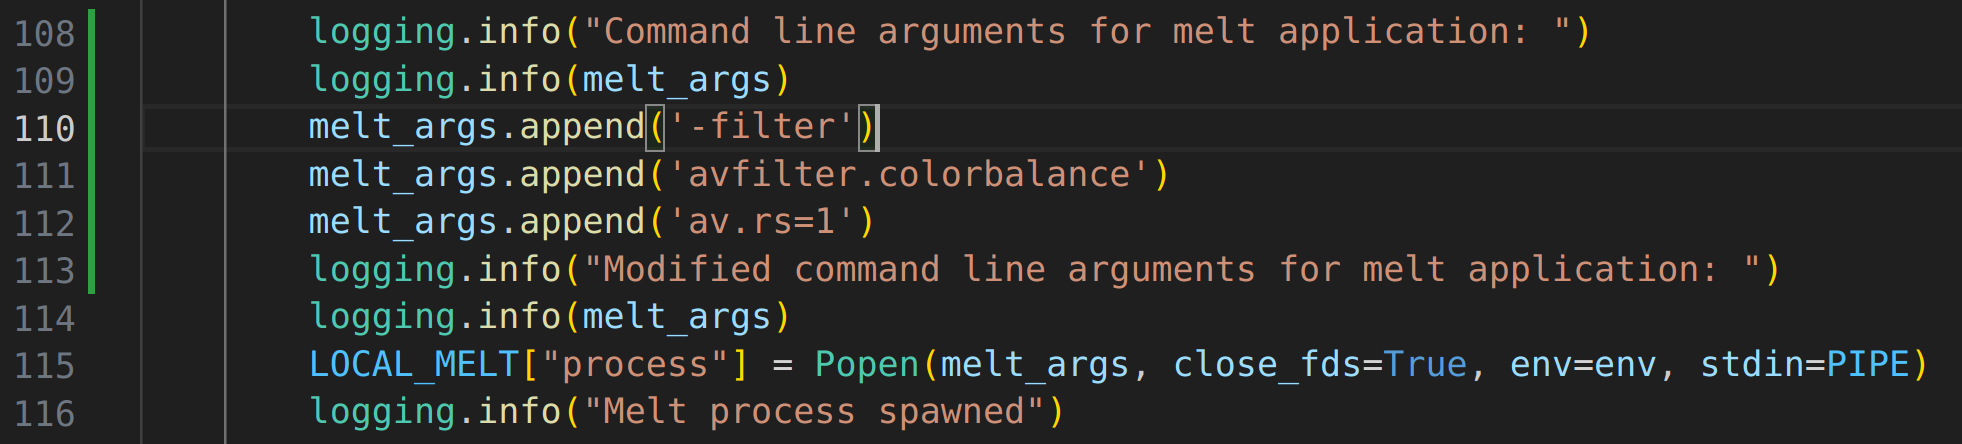
\includegraphics[height=0.13\textwidth]{code.png}
	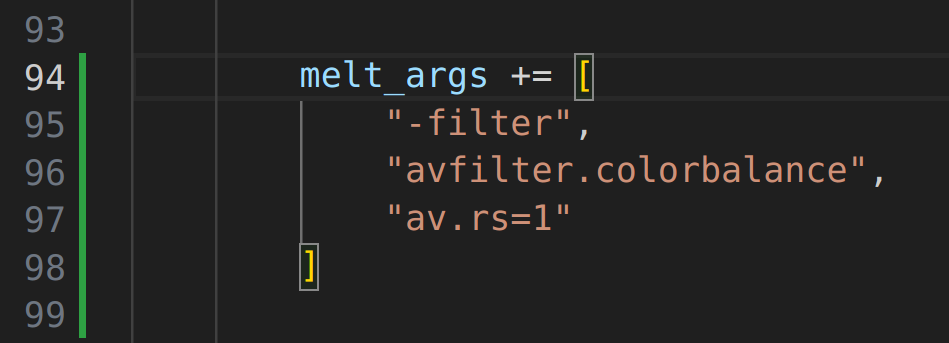
\includegraphics[height=0.13\textwidth]{codecleaner.png}
\end{center}

\begin{center}
	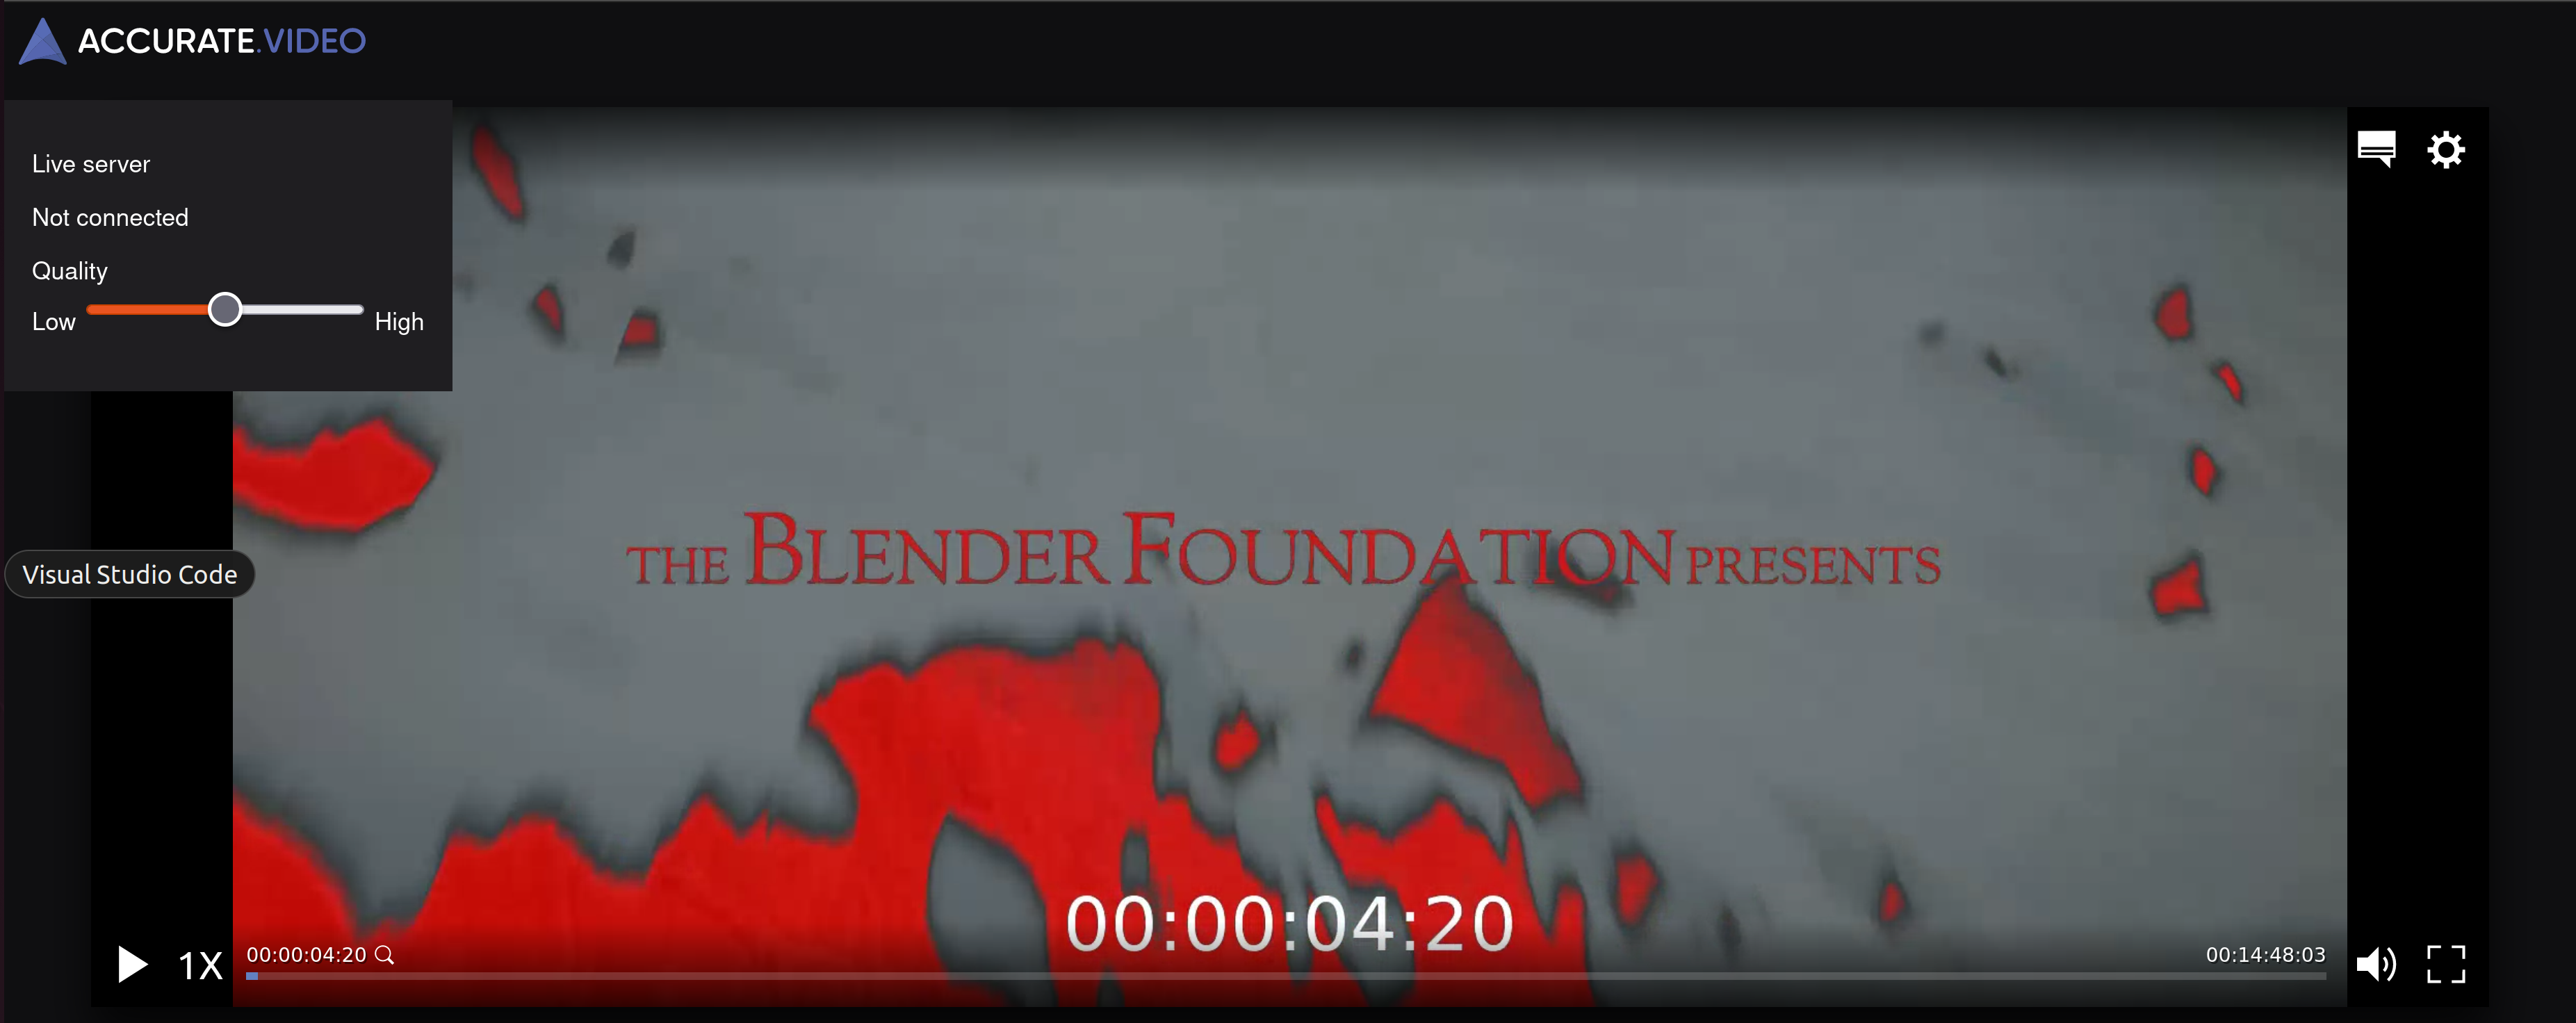
\includegraphics[width=0.8\textwidth]{ap_red.png}
\end{center}









%-------------------------------------------------------------------------------------------------------
\subsubsection*{Video Transcoding} 

Transcoding is the conversion of one digital data format into another.~\cite{transcoding}







%-------------------------------------------------------------------------------------------------------
\subsubsection*{Video Compression with h.264} 
% Explain WebRTC

\begin{CountingDefinition}[h.264]{def:h264}
	
	h.264 refers to a video compression standard. In the context of real-time communication, h.264 is one of the video codecs that can be used to compress and decompress video streams.
	
\end{CountingDefinition}









%-------------------------------------------------------------------------------------------------------
\subsubsection*{WebRTC} 
% Explain WebRTC

\begin{CountingDefinition}[WebRTC]{def:WebRTC}
	
	Web Real-Time Communication (WebRTC), is a free, open-source project that provides web browsers and mobile applications with real-time communication. It enables direct communication between browsers or applications, allowing for peer-to-peer communication without the need for intermediary servers in certain scenarios.
	
\end{CountingDefinition}

WebRTC supports various video codecs, and h.264 is popular due to its efficiency in compressing video data while maintaining good quality. It is widely used for video conferencing, streaming, and other real-time communication applications. The video streams exchanged between the browser and the backend are encoded and decoded using h.264.






%-------------------------------------------------------------------------------------------------------
\subsubsection*{Audio Video Interleave} 

Audio Video Interleave (AVI) is a file format that can contain audio and video information to allow synchronized playback of audio and video components. 
It is a container format, which means that it can contain multiple streams of audio and video data, along with other multimedia data such as subtitles.~\cite{avi}












%-------------------------------------------------------------------------------------------------------
\subsubsection*{Named Pipe} 

A named pipe is a type of interprocess communication (IPC) mechanism. It provides a way for processes to pass data to each other and it is bidirectional. 
Named pipes follow a First-In-First-Out (FIFO) structure: The first data written into the pipe is the first data to be read. This maintains a sequential order for data transmission.
A traditional pipe is \textit{unnamed} and terminates when its process terminates. A named pipe can last beyond the life of the process, as long as the system is running.~\cite{namedpipe}









%-------------------------------------------------------------------------------------------------------
\subsubsection*{REST} 


Representational State Transfer (REST) is an architectural style for designing networked applications. A REST Application Programming Interface (API) exposes a set of endpoints (URLs) that allow communication between different software systems over the internet and it uses the hypertext transfer protocol (HTTP) methods.~\cite{IEEE_Rest, webservice, Nodejs_Rest}











%-------------------------------------------------------------------------------------------------------
\subsubsection*{JIT} 
%
\begin{CountingDefinition}[JIT]{def:JIT}
	
	JIT (Just-In-Time), in the context of video files for streaming, refers to a dynamic software solution employed for real-time video transformation on a server. It is used for on-the-fly conversion of video files, optimizing them for streaming. The process includes the transformation of a video file, potentially one with non-web-friendly formats, into a more suitable format for the playback in web browsers.
	
\end{CountingDefinition}






	
	
	
	
\end{document}